\documentclass[border=8pt]{standalone}
\usepackage{amsmath,amssymb,bm}
\usepackage{xcolor}
\usepackage{tikz}
% --- accent pair: meson table = deck purple, baryon table = deck orange (deepened for white text) ---
\definecolor{P}{HTML}{A8500B}    % entry text (dark orange)
\definecolor{H}{HTML}{C8650F}    % header bar
\definecolor{band}{HTML}{FDF1E4}% soft tint for alternate rows
\definecolor{rule}{HTML}{F0CBA3} % light separator

% column centres (cm) and geometry -- identical to the meson table
\newcommand{\cA}{2.3}\newcommand{\cB}{6.1}\newcommand{\cC}{9.0}\newcommand{\cD}{11.5}\newcommand{\cE}{13.5}
\newcommand{\Wd}{14.6}     % table width
\newcommand{\Hh}{1.3}      % header height
\newcommand{\Rh}{1.0}      % row height
\newcommand{\Nr}{7}        % number of body rows

% \row{i}{baryon}{mass}{J^P}{I}{S}   (i = body row)
\newcommand{\row}[6]{%
  \pgfmathsetmacro{\yy}{-(\Hh+(#1-0.5)*\Rh)}%
  \node[text=P] at (\cA,\yy) {#2};
  \node at (\cB,\yy) {#3};
  \node at (\cC,\yy) {#4};
  \node at (\cD,\yy) {#5};
  \node at (\cE,\yy) {#6};}
\newcommand{\band}[2]{\fill[band] (0,{-(\Hh+(#1-1)*\Rh)}) rectangle (\Wd,{-(\Hh+#2*\Rh)});}
\newcommand{\sep}[1]{\draw[rule,line width=.6pt] (0,{-(\Hh+#1*\Rh)}) -- (\Wd,{-(\Hh+#1*\Rh)});}

\begin{document}
\Large
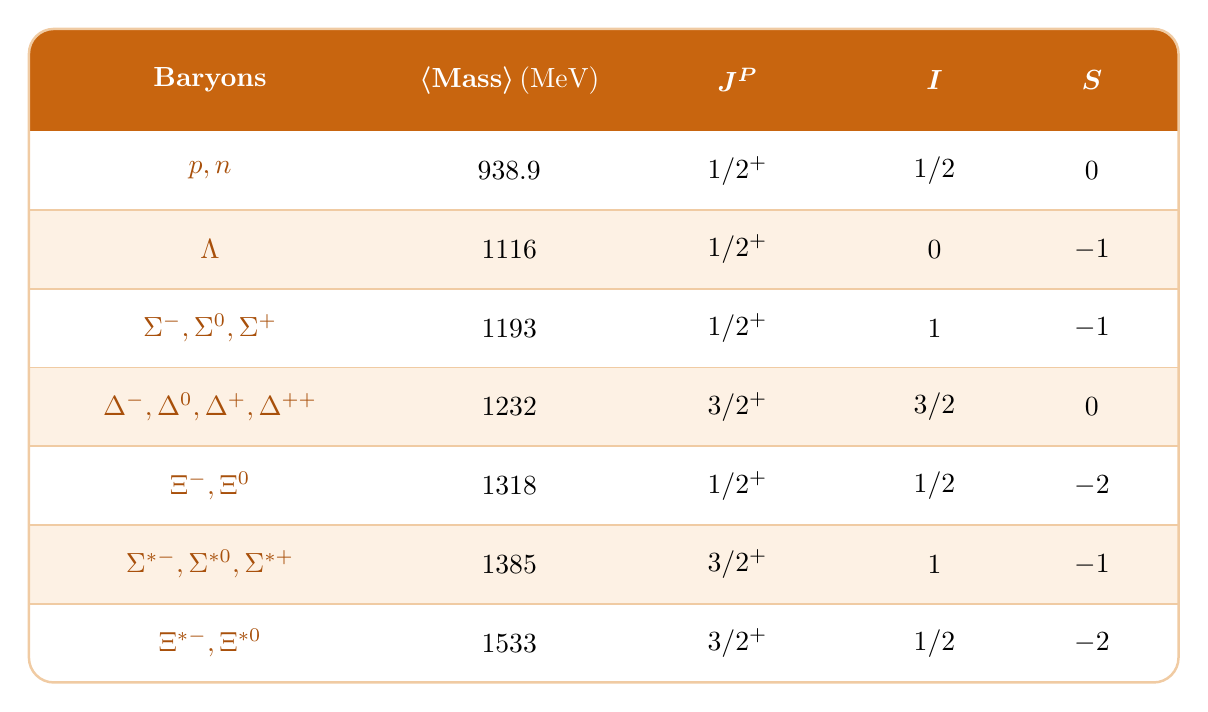
\begin{tikzpicture}
  \pgfmathsetmacro{\Ht}{\Hh+\Nr*\Rh}
  % ---- backgrounds, clipped to a rounded rectangle ----
  \begin{scope}
    \clip[rounded corners=9pt] (0,0) rectangle (\Wd,-\Ht);
    \fill[H] (0,0) rectangle (\Wd,-\Hh);              % header bar
    \band{2}{2}\band{4}{4}\band{6}{6}                 % alternate rows
  \end{scope}
  % ---- separators ----
  \sep{1}\sep{2}\sep{3}\sep{4}\sep{5}\sep{6}
  \draw[rule,line width=.9pt,rounded corners=9pt] (0,0) rectangle (\Wd,-\Ht);
  % ---- header text ----
  \node[text=white] at (\cA,-\Hh/2) {\bfseries Baryons};
  \node[text=white] at (\cB,-\Hh/2) {$\bm{\langle}\textbf{Mass}\bm{\rangle}$\,{\normalsize\mdseries(MeV)}};
  \node[text=white] at (\cC,-\Hh/2) {$\bm{J^{P}}$};
  \node[text=white] at (\cD,-\Hh/2) {$\bm{I}$};
  \node[text=white] at (\cE,-\Hh/2) {$\bm{S}$};
  % ---- body ----
  \row{1}{$p,n$}{$938.9$}{$1/2^{+}$}{$1/2$}{$0$}
  \row{2}{$\Lambda$}{$1116$}{$1/2^{+}$}{$0$}{$-1$}
  \row{3}{$\Sigma^-,\Sigma^0,\Sigma^+$}{$1193$}{$1/2^{+}$}{$1$}{$-1$}
  \row{4}{$\Delta^-,\Delta^0,\Delta^+,\Delta^{++}$}{$1232$}{$3/2^{+}$}{$3/2$}{$0$}
  \row{5}{$\Xi^-,\Xi^0$}{$1318$}{$1/2^{+}$}{$1/2$}{$-2$}
  \row{6}{$\Sigma^{*-},\Sigma^{*0},\Sigma^{*+}$}{$1385$}{$3/2^{+}$}{$1$}{$-1$}
  \row{7}{$\Xi^{*-},\Xi^{*0}$}{$1533$}{$3/2^{+}$}{$1/2$}{$-2$}
\end{tikzpicture}
\end{document}
